%\documentstyle[epsf,twocolumn]{jarticle}       %LaTeX2e仕様
\documentclass[twocolumn]{jarticle}     %pLaTeX2e仕様(platex.exeの場合)
% \documentclass[onecolumn]{ujarticle}   %pLaTeX2e仕様(uplatex.exeの場合)
%%%%%%%%%%%%%%%%%%%%%%%%%%%%%%%%%%%%%%%%%%%%%%%%%%%%%%%%%%%%%%
%%
%%  基本バージョン
%%
%%%%%%%%%%%%%%%%%%%%%%%%%%%%%%%%%%%%%%%%%%%%%%%%%%%%%%%%%%%%%%%%
\setlength{\topmargin}{-45pt}
%\setlength{\oddsidemargin}{0cm}
\setlength{\oddsidemargin}{-7.5mm}
%\setlength{\evensidemargin}{0cm}
\setlength{\textheight}{24.1cm}
%setlength{\textheight}{25cm}
\setlength{\textwidth}{17.4cm}
%\setlength{\textwidth}{172mm}
\setlength{\columnsep}{11mm}

%\kanjiskip=.07zw plus.5pt minus.5pt


% 【節が変わるごとに (1.1)(1.2) … (2.1)(2.2) と数式番号をつけるとき】
%\makeatletter
%\renewcommand{\theequation}{%
%\thesection.\arabic{equation}} %\@addtoreset{equation}{section}
%\makeatother

%\renewcommand{\arraystretch}{0.95} 行間の設定
%%%%%%%%%%%%%%%%%%%%%%%%%%%%%%%%%%%%%%%%%%%%%%%%%%%%%%%%
%\usepackage{graphicx}   %pLaTeX2e仕様(\documentstyle ->\documentclass)
\usepackage[dvipdfmx]{graphicx}
\usepackage{subcaption}
\usepackage{multirow}
\usepackage{amsmath}
\usepackage{url}
\usepackage{ulem}
\usepackage{algorithm}
\usepackage{algorithmic}
\usepackage{listings} %,jlisting} %日本語のコメントアウトをする場合jlistingが必要
%ここからソースコードの表示に関する設定
\lstset{
  basicstyle={\ttfamily},
  identifierstyle={\small},
  commentstyle={\smallitshape},
  keywordstyle={\small\bfseries},
  ndkeywordstyle={\small},
  stringstyle={\small\ttfamily},
  frame={tb},
  breaklines=true,
  columns=[l]{fullflexible},
  numbers=left,
  xrightmargin=0zw,
  xleftmargin=3zw,
  numberstyle={\scriptsize},
  stepnumber=1,
  numbersep=1zw,
  lineskip=-0.5ex
}
%%%%%%%%%%%%%%%%%%%%%%%%%%%%%%%%%%%%%%%%%%%%%%%%%%%%%%%%
\begin{document}

	%bibtex用の設定
	%\bibliographystyle{ujarticle}

	\twocolumn[
		\noindent
		\hspace{1em}
		2020 年 7 月 24 日
		ゼミ資料
		\hfill
		B4 杉山 竜弥
		\vspace{2mm}

		\hrule
		\begin{center}
			{\Large \bf 進捗報告}
		\end{center}
		\hrule
		\vspace{9mm}
	]

	% ‚ここから 文章 Start!
\section{今週やったこと}
\begin{itemize}
	\item {NASの実装}
\end{itemize}

\section{NAS}
\subsection{設定}
図\ref{fig:model}には実験で用いた探索中のセルの構造を,
表\ref{tab:setting}には実験設定を示した.
入力・出力ノードの数は, ともに1に設定した.
また出力ノードへの接続はチャンネルのconcatであり, 今回は3つのノードを使ってチャンネル数を3倍にした.
ノードは7にしたため, 探索する辺は15となった.
表\ref{tab:ops}のように, 畳み込み層, プーリング層, 恒等写像, 零写像の6つの演算子を用意した.
またセルの入力は, チャンネル数の前処理としてReLU-Conv-BNを用いた.

このセルを4つ重ねたものを用いて, Cifar10の10クラス分類器を構築した.
モデルのOptimizerはSDGで, アーキテクチャを表す\thetaはAdamとした.

\subsection{実験}
実験ではまず\thetaを固定して演算子ごとの重みだけを(a)30 epoch学習し,
その後\thetaも加えて(b)60 epoch訓練した.
得られた\thetaからセルの構造を決定し, 重みを(c)90 epochで再学習した.
(Accuracyのグラフを載せたかったのですが, 時間が足りませんでした...)
(a)で50\%, (b)で66.8\%, (c)で最大66.8\%となった.
訓練時間は全体でおよそ2~3時間?程度であった.

図\ref{fig:cell}に得られたセルを示した.
このセルの場合モデル全体では, 前処理も含めて10層に相当する.
使用された演算子はConv5x5とMaxPoolとなった.
画像識別にしばしばみられる妥当な構成と思われる.

\section{考察}
アーキテクチャを決定するアルゴリズム
\begin{enumerate}
  \item 辺ごとに最尤の演算子1つを決定\\
  零写像を対等に扱ったため, グラフが切断される場合があり識別できなくなった.
  \item ノードごとに(零写像を除く)最尤の演算子を持つ辺に決定\\
  ノードが必ず親を持つため連結が保証された.
  今回は1入力であるため, 全ての中間ノードは1つの親ノードを持つように設定した.
\end{enumerate}

初期段階で1.のアルゴリズムを実装したが, うまくいかなかったため論文\cite{DBLP:journals/corr/abs-1806-09055}のコードを参考に2.に変更した.
しかしノードの親の数が固定されることになった.
元論文のように入力ノードを2つにすることで, より複雑なアーキテクチャを表現することを試したい.

今回は実装できなかった, Reduction Cellと呼ぶstride=2のセルを導入して精度の改善を目指したい.

\begin{table}[tb]
  \begin{center}
    \caption{実験の設定}
    \begin{tabular}{|c|c|} \hline
      Cell & 4 \\ \hline
      Node & 7(input=1, output=1) \\ \hline
      Optim(model) & SDG(lr=5e-3, momentum=0.9) \\ \hline
      Optim($\theta$) & Adam(lr=5e-4, $\beta$=(0.5, 0.999)) \\ \hline
      Loss & Cross Entropy Loss \\ \hline
      batch size & 64 \\ \hline
      train data & 8000 \\ \hline
      epoch & 30+60+90 \\ \hline
    \end{tabular}
    \label{tab:setting}
  \end{center}
\end{table}

\begin{table}[tb]
  \begin{center}
    \caption{演算子候補}
    \begin{tabular}{|c|} \hline
      \verb|conv_3x3| \\ \hline
      \verb|conv_5x5| \\ \hline
      \verb|avg_pool_3x3| \\ \hline
      \verb|max_pool_3x3| \\ \hline
      \verb|skip_connect| \\ \hline
      \verb|none| \\ \hline
    \end{tabular}
    \label{tab:ops}
  \end{center}
\end{table}

\begin{figure}[tb]
	\begin{center}
		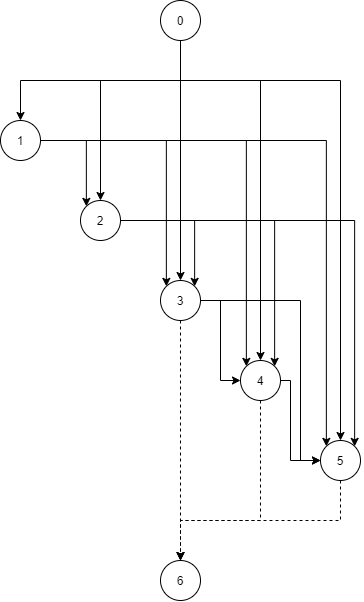
\includegraphics[clip,width=8.5cm]{search.png}
		\caption{セルの全体構造}
		\label{fig:model}
	\end{center}
\end{figure}

\begin{figure}[tb]
	\begin{center}
		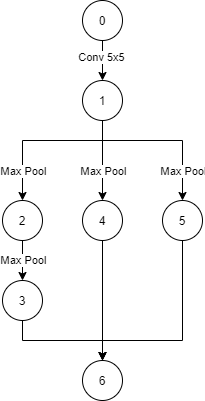
\includegraphics[clip,width=7.5cm]{normal.png}
		\caption{探索したセル}
		\label{fig:cell}
	\end{center}
\end{figure}

\section{今後の予定}
% なんとなくなんかの勉強をするとかではなく具体的に
\begin{itemize}
  \item 複数入力のセルの実装
  \item Reductionセルの実装
\end{itemize}


\section{ソースコード}
% 埋め込みでもGitでもいいので参照できるように
Githubの同階層の\url{NAS_test.ipynb}を参照してください.
% \url{https://github.com/tatsuya-sugiyama/WeeklyReport/blob/2020_0717/report/2020_07_17/NAS_test.ipynb}
%
% \begin{lstlisting}[caption=Edge,label=Edge]

% \end{lstlisting}

\section{付録}
表\ref{tab:theta}に$\theta$の結果を示した.
初期値0から学習し, 辺ごとにSoftMaxで確率分布にする.
この結果からアーキテクチャを構築した.

\begin{table*}[tb]
  \begin{center}
    \caption{(付録)$\theta$の結果\\
      縦軸が(0, 1), (0, 2),...などの辺, 横軸が演算子.}
    \begin{tabular}{|c|c|c|c|c|c|} \hline
      \verb|conv_3x3| & \verb|conv_5x5| & \verb|avg_pool_3x3| & \verb|max_pool_3x3| & \verb|skip_connect| & \verb|none| \\ \hline
      0.0183 & 0.0447 & -0.0951 & -0.0092 & 0.016 & -0.0878 \\ \hline
      -0.0608 & 0.0019 & -0.0622 & 0.0613 & 0.0152 & 0.0838 \\ \hline
      -0.0071 & 0.0016 & -0.0772 & 0.0199 & 0.0493 & 0.0382 \\ \hline
      0.0321 & 0.0254 & -0.0595 & -0.0185 & -0.0134 & 0.0269 \\ \hline
      0.0043 & 0.0371 & -0.0482 & -0.0454 & -0.0018 & 0.0304 \\ \hline
      -0.0868 & 0.0845 & -0.4144 & 0.4559 & -0.3905 & -0.1644 \\ \hline
      0.0053 & 0.0941 & -0.3314 & 0.2671 & -0.2094 & -0.0193 \\ \hline
      -0.0009 & 0.053 & -0.3054 & 0.2834 & -0.2829 & -0.016 \\ \hline
      0.0286 & 0.1113 & -0.2692 & 0.1651 & -0.2161 & 0.0021 \\ \hline
      -0.0434 & 0.008 & -0.2832 & 0.3248 & -0.1618 & -0.0383 \\ \hline
      0.0012 & 0.0817 & -0.2243 & 0.1887 & -0.214 & -0.0307 \\ \hline
      0.0144 & 0.0216 & -0.2078 & 0.1623 & -0.1393 & 0.0263 \\ \hline
      0.0239 & 0.0498 & -0.1619 & 0.1491 & -0.1734 & -0.0266 \\ \hline
      0.0325 & 0.0618 & -0.1066 & -0.0367 & -0.0554 & 0.0913 \\ \hline
      0.0211 & 0.1379 & -0.1649 & -0.0872 & -0.129 & 0.0195 \\ \hline
    \end{tabular}
    \label{tab:theta}
  \end{center}
\end{table*}

% 参考文献リスト
\bibliographystyle{unsrt}
\bibliography{ref}
\end{document}
